\tikzset{every picture/.style={line width=0.75pt}} %set default line width to 0.75pt        

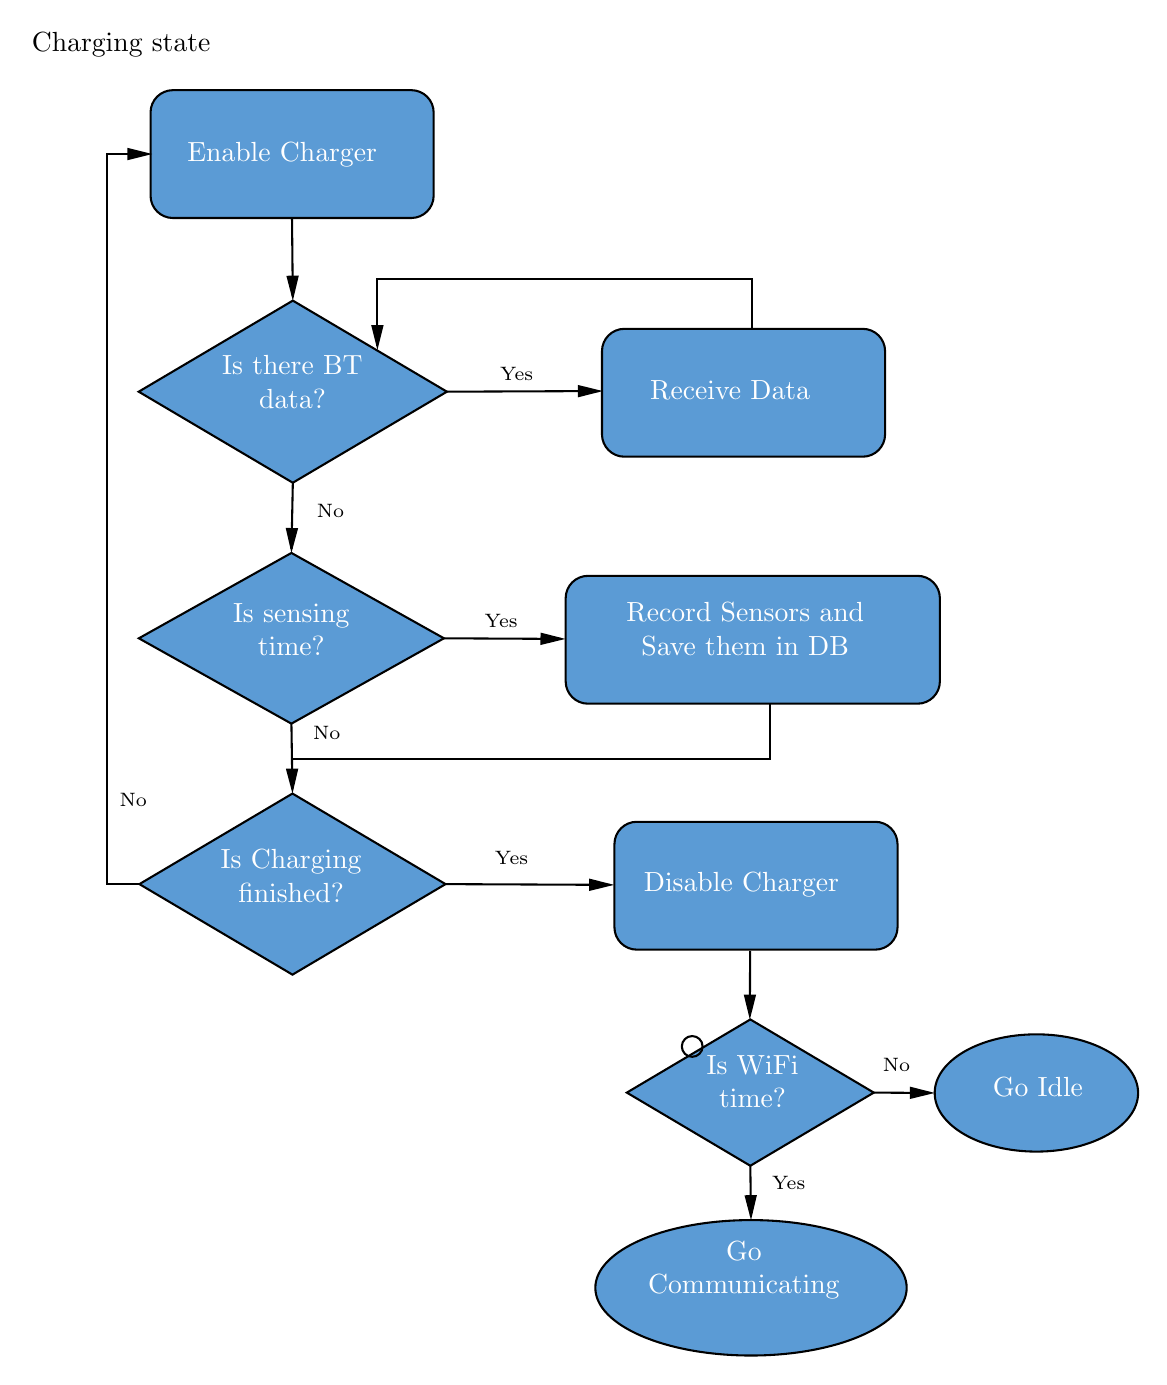
\begin{tikzpicture}[x=0.75pt,y=0.75pt,yscale=-1,xscale=1]
%uncomment if require: \path (0,680); %set diagram left start at 0, and has height of 680

%Flowchart: Alternative Process [id:dp6196306459310315] 
\draw  [fill={rgb, 255:red, 91; green, 155; blue, 213 }  ,fill opacity=1 ] (70.7,53.38) .. controls (70.7,47.43) and (75.53,42.6) .. (81.48,42.6) -- (196.32,42.6) .. controls (202.27,42.6) and (207.1,47.43) .. (207.1,53.38) -- (207.1,93.42) .. controls (207.1,99.37) and (202.27,104.2) .. (196.32,104.2) -- (81.48,104.2) .. controls (75.53,104.2) and (70.7,99.37) .. (70.7,93.42) -- cycle ;
%Flowchart: Alternative Process [id:dp26981305808222733] 
\draw  [fill={rgb, 255:red, 91; green, 155; blue, 213 }  ,fill opacity=1 ] (288.2,168.38) .. controls (288.2,162.43) and (293.03,157.6) .. (298.98,157.6) -- (413.82,157.6) .. controls (419.77,157.6) and (424.6,162.43) .. (424.6,168.38) -- (424.6,208.42) .. controls (424.6,214.37) and (419.77,219.2) .. (413.82,219.2) -- (298.98,219.2) .. controls (293.03,219.2) and (288.2,214.37) .. (288.2,208.42) -- cycle ;
%Flowchart: Alternative Process [id:dp5186412191236014] 
\draw  [fill={rgb, 255:red, 91; green, 155; blue, 213 }  ,fill opacity=1 ] (270.7,287.38) .. controls (270.7,281.43) and (275.53,276.6) .. (281.48,276.6) -- (440.22,276.6) .. controls (446.17,276.6) and (451,281.43) .. (451,287.38) -- (451,327.42) .. controls (451,333.37) and (446.17,338.2) .. (440.22,338.2) -- (281.48,338.2) .. controls (275.53,338.2) and (270.7,333.37) .. (270.7,327.42) -- cycle ;
%Flowchart: Alternative Process [id:dp5155190585787537] 
\draw  [fill={rgb, 255:red, 91; green, 155; blue, 213 }  ,fill opacity=1 ] (294.2,405.88) .. controls (294.2,399.93) and (299.03,395.1) .. (304.98,395.1) -- (419.82,395.1) .. controls (425.77,395.1) and (430.6,399.93) .. (430.6,405.88) -- (430.6,445.92) .. controls (430.6,451.87) and (425.77,456.7) .. (419.82,456.7) -- (304.98,456.7) .. controls (299.03,456.7) and (294.2,451.87) .. (294.2,445.92) -- cycle ;
%Flowchart: Decision [id:dp9466964444778403] 
\draw  [fill={rgb, 255:red, 91; green, 155; blue, 213 }  ,fill opacity=1 ] (138.57,265.57) -- (212.07,306.7) -- (138.57,347.82) -- (65.07,306.7) -- cycle ;
%Flowchart: Decision [id:dp9415932298575294] 
\draw  [fill={rgb, 255:red, 91; green, 155; blue, 213 }  ,fill opacity=1 ] (139.25,144) -- (213.5,187.88) -- (139.25,231.75) -- (65,187.88) -- cycle ;
%Flowchart: Decision [id:dp8462922917717295] 
\draw  [fill={rgb, 255:red, 91; green, 155; blue, 213 }  ,fill opacity=1 ] (139.08,381.5) -- (212.83,425.13) -- (139.08,468.75) -- (65.33,425.13) -- cycle ;
%Flowchart: Decision [id:dp77955690329976] 
\draw  [fill={rgb, 255:red, 91; green, 155; blue, 213 }  ,fill opacity=1 ] (359.67,490.33) -- (419.17,525.58) -- (359.67,560.83) -- (300.17,525.58) -- cycle ;
%Shape: Ellipse [id:dp29148240310091045] 
\draw  [fill={rgb, 255:red, 91; green, 155; blue, 213 }  ,fill opacity=1 ] (448.5,525.75) .. controls (448.5,510.15) and (470.44,497.5) .. (497.5,497.5) .. controls (524.56,497.5) and (546.5,510.15) .. (546.5,525.75) .. controls (546.5,541.35) and (524.56,554) .. (497.5,554) .. controls (470.44,554) and (448.5,541.35) .. (448.5,525.75) -- cycle ;
%Shape: Ellipse [id:dp19636835563793276] 
\draw  [fill={rgb, 255:red, 91; green, 155; blue, 213 }  ,fill opacity=1 ] (285,619.63) .. controls (285,601.61) and (318.58,587) .. (360,587) .. controls (401.42,587) and (435,601.61) .. (435,619.63) .. controls (435,637.64) and (401.42,652.25) .. (360,652.25) .. controls (318.58,652.25) and (285,637.64) .. (285,619.63) -- cycle ;
%Straight Lines [id:da5943950824854729] 
\draw    (138.86,104.43) -- (139.23,142) ;
\draw [shift={(139.25,144)}, rotate = 269.43] [fill={rgb, 255:red, 0; green, 0; blue, 0 }  ][line width=0.08]  [draw opacity=0] (12,-3) -- (0,0) -- (12,3) -- cycle    ;
%Straight Lines [id:da7907623475138235] 
\draw    (213.5,187.88) -- (286.57,187.58) ;
\draw [shift={(288.57,187.57)}, rotate = 539.77] [fill={rgb, 255:red, 0; green, 0; blue, 0 }  ][line width=0.08]  [draw opacity=0] (12,-3) -- (0,0) -- (12,3) -- cycle    ;
%Straight Lines [id:da07377950817301082] 
\draw    (139.25,231.75) -- (138.61,263.57) ;
\draw [shift={(138.57,265.57)}, rotate = 271.15] [fill={rgb, 255:red, 0; green, 0; blue, 0 }  ][line width=0.08]  [draw opacity=0] (12,-3) -- (0,0) -- (12,3) -- cycle    ;
%Straight Lines [id:da9328725883574844] 
\draw    (212.07,306.7) -- (268.57,306.99) ;
\draw [shift={(270.57,307)}, rotate = 180.3] [fill={rgb, 255:red, 0; green, 0; blue, 0 }  ][line width=0.08]  [draw opacity=0] (12,-3) -- (0,0) -- (12,3) -- cycle    ;
%Straight Lines [id:da6867836679961588] 
\draw    (138.57,347.82) -- (139.05,379.5) ;
\draw [shift={(139.08,381.5)}, rotate = 269.13] [fill={rgb, 255:red, 0; green, 0; blue, 0 }  ][line width=0.08]  [draw opacity=0] (12,-3) -- (0,0) -- (12,3) -- cycle    ;
%Shape: Right Angle [id:dp5058488629689668] 
\draw   (369,338.5) -- (369,364.66) -- (138.83,364.66) ;
%Straight Lines [id:da7200309232689854] 
\draw    (212.83,425.13) -- (292,425.49) ;
\draw [shift={(294,425.5)}, rotate = 180.26] [fill={rgb, 255:red, 0; green, 0; blue, 0 }  ][line width=0.08]  [draw opacity=0] (12,-3) -- (0,0) -- (12,3) -- cycle    ;
%Straight Lines [id:da19815213231327156] 
\draw    (359.57,457.29) -- (359.45,488.33) ;
\draw [shift={(359.44,490.33)}, rotate = 270.22] [fill={rgb, 255:red, 0; green, 0; blue, 0 }  ][line width=0.08]  [draw opacity=0] (12,-3) -- (0,0) -- (12,3) -- cycle    ;
%Straight Lines [id:da8355990256873418] 
\draw    (419.17,525.58) -- (446.5,525.74) ;
\draw [shift={(448.5,525.75)}, rotate = 180.33] [fill={rgb, 255:red, 0; green, 0; blue, 0 }  ][line width=0.08]  [draw opacity=0] (12,-3) -- (0,0) -- (12,3) -- cycle    ;
%Straight Lines [id:da9207583345712389] 
\draw    (359.67,560.83) -- (359.97,585) ;
\draw [shift={(360,587)}, rotate = 269.27] [fill={rgb, 255:red, 0; green, 0; blue, 0 }  ][line width=0.08]  [draw opacity=0] (12,-3) -- (0,0) -- (12,3) -- cycle    ;
%Shape: Right Angle [id:dp15735173819795922] 
\draw   (179.5,133.8) -- (360.6,133.8) -- (360.6,157.2) ;
%Straight Lines [id:da905292498462269] 
\draw    (180,133.8) -- (180,165.8) ;
\draw [shift={(180,167.8)}, rotate = 270] [fill={rgb, 255:red, 0; green, 0; blue, 0 }  ][line width=0.08]  [draw opacity=0] (12,-3) -- (0,0) -- (12,3) -- cycle    ;
%Shape: Right Angle [id:dp7630273915612096] 
\draw   (65.33,425.13) -- (49.75,425.13) -- (49.75,72.88) ;
%Straight Lines [id:da48930415284774065] 
\draw    (49.75,73.38) -- (69.5,73.38) ;
\draw [shift={(71.5,73.38)}, rotate = 180] [fill={rgb, 255:red, 0; green, 0; blue, 0 }  ][line width=0.08]  [draw opacity=0] (12,-3) -- (0,0) -- (12,3) -- cycle    ;

% Text Node
\draw (12,13) node [anchor=north west][inner sep=0.75pt]   [align=left] {Charging state};
% Text Node
\draw (86.9,66) node [anchor=north west][inner sep=0.75pt]   [align=left] {\textcolor[rgb]{1,1,1}{Enable Charger}};
% Text Node
\draw (309.9,181) node [anchor=north west][inner sep=0.75pt]   [align=left] {\textcolor[rgb]{1,1,1}{Receive Data}};
% Text Node
\draw (291.9,288) node [anchor=north west][inner sep=0.75pt]   [align=left] {\begin{minipage}[lt]{95.71pt}\setlength\topsep{0pt}
\begin{center}
\textcolor[rgb]{1,1,1}{Record Sensors and}\\\textcolor[rgb]{1,1,1}{Save them in DB}
\end{center}

\end{minipage}};
% Text Node
\draw (306.9,418) node [anchor=north west][inner sep=0.75pt]   [align=left] {\textcolor[rgb]{1,1,1}{Disable Charger}};
% Text Node
\draw (102.5,169) node [anchor=north west][inner sep=0.75pt]  [color={rgb, 255:red, 255; green, 255; blue, 255 }  ,opacity=1 ] [align=left] {\begin{minipage}[lt]{52.6pt}\setlength\topsep{0pt}
\begin{center}
Is there BT\\data?
\end{center}

\end{minipage}};
% Text Node
\draw (104.57,288.57) node [anchor=north west][inner sep=0.75pt]  [color={rgb, 255:red, 255; green, 255; blue, 255 }  ,opacity=1 ] [align=left] {\begin{minipage}[lt]{48.65pt}\setlength\topsep{0pt}
\begin{center}
Is sensing\\time?
\end{center}

\end{minipage}};
% Text Node
\draw (100.33,407) node [anchor=north west][inner sep=0.75pt]  [color={rgb, 255:red, 255; green, 255; blue, 255 }  ,opacity=1 ] [align=left] {\begin{minipage}[lt]{54.89pt}\setlength\topsep{0pt}
\begin{center}
Is Charging\\finished?
\end{center}

\end{minipage}};
% Text Node
\draw (237.57,174.71) node [anchor=north west][inner sep=0.75pt]  [font=\scriptsize] [align=left] {Yes};
% Text Node
\draw (149.29,240.43) node [anchor=north west][inner sep=0.75pt]  [font=\scriptsize] [align=left] {No};
% Text Node
\draw (230.14,293.57) node [anchor=north west][inner sep=0.75pt]  [font=\scriptsize] [align=left] {Yes};
% Text Node
\draw (147.48,347.57) node [anchor=north west][inner sep=0.75pt]  [font=\scriptsize] [align=left] {No};
% Text Node
\draw (235.14,407.67) node [anchor=north west][inner sep=0.75pt]  [font=\scriptsize] [align=left] {Yes};
% Text Node
\draw (336.67,506.33) node [anchor=north west][inner sep=0.75pt]  [color={rgb, 255:red, 255; green, 255; blue, 255 }  ,opacity=1 ] [align=left] {\begin{minipage}[lt]{33.88pt}\setlength\topsep{0pt}
\begin{center}
Is WiFi\\time?
\end{center}

\end{minipage}};
% Text Node
\draw (473,516.5) node [anchor=north west][inner sep=0.75pt]  [color={rgb, 255:red, 255; green, 255; blue, 255 }  ,opacity=1 ] [align=left] {\begin{minipage}[lt]{35.62pt}\setlength\topsep{0pt}
\begin{center}
Go Idle
\end{center}

\end{minipage}};
% Text Node
\draw (306,596) node [anchor=north west][inner sep=0.75pt]  [color={rgb, 255:red, 255; green, 255; blue, 255 }  ,opacity=1 ] [align=left] {\begin{minipage}[lt]{73.59pt}\setlength\topsep{0pt}
\begin{center}
Go\\Communicating
\end{center}

\end{minipage}};
% Text Node
\draw (368.67,564.33) node [anchor=north west][inner sep=0.75pt]  [font=\scriptsize] [align=left] {Yes};
% Text Node
\draw (422,507.67) node [anchor=north west][inner sep=0.75pt]  [font=\scriptsize] [align=left] {No};
% Text Node
\draw (54.29,380) node [anchor=north west][inner sep=0.75pt]  [font=\scriptsize] [align=left] {No};

\draw   (331.67, 503.33) circle [x radius= 5, y radius= 5]   ;
\end{tikzpicture}